\chapter{Data analysis and Event reconstruction}\label{section:Reconstruction}

In this chapter, we will first explain the event selection, then how we apply the truth matching, traditional reconstruct method, and the machine learning approach.

\section{Data analysis}\label{sec:Data analysis}

\subsection{Event selection}\label{subsec:Event selection}
The top all hadronic decay channel has 2 b-jets and 4 quark jets, all of them in our configuration are not in the boosted region, that means the daughters of top quarks will not appear with high transverse momentum. Following the event selection used in the \cite{Mccarthy:2015ucy},  we apply a event selection that an event should at least exists \textbf{2 b-jets} and \textbf{4 quark jets} satisfied $p_{\rm T}$ larger than \textbf{25 GeV} and $|\eta|$ less than \textbf{2.5}. A cutflow table and figure can help us to understand how many events are killed by the selections. We may apply 5 cuts and see the evolution of surviving event numbers. The rule of cuts is shown in Table \ref{table:cuts}, and the cutflow is shown in Figure \ref{fig:cutflow}.
\\
\begin{center}
	\begin{table}[h]
		\begin{tabular}{p{0.1\textwidth} c c c }
			\cline{1-3}
			\#Cut    & Number of b-jets & Number of quark jets  \\
			\hline
			C1      &   0  & 4    \\
			C2      &   0  & 5    \\
			C3      &   0  & 6    \\
			C4      &   1  & 6    \\
			C5      &   2  & 6    \\
			\hline
		\end{tabular}
		\caption{Rule of cuts. All the cuts require a kinematic limitation that $p_{T} > 25$ GeV and $|\eta|<2.5$.}
		\label{table:cuts}
	\end{table}
\end{center}
The b-tagging and jet information we used here is provided by the Delphes, a detector simulation package.\cite{deFavereau:2013fsa} The b-tagging is a method of jet flavor tagging used in CMS and ATLAS.\cite{ATLAS:2016gsw}\cite{Sirunyan:2017ezt} This method base on the b-hadron properties, such as the displaced vertex from the primary vertex, large b-hadron mass, large impact parameters(d0), and semi-leptonic e/$\mu$ decay of B-hadron. This is also related to the track reconstruction and secondary vertex reconstruction. The Delphes package decide a jet is b-tagged or not based on an efficiency table and returns an array to indicate a jet is b-tagged or not.
\\
The number of surviving events is an important factor in our event generation. If the survived events are very rare, it means our cuts are too tight that may also ignore the events we want. Also, the lack of surviving events may slow down our data generation efficiency. In Figure \ref{fig:cutflow}, it shows that there are around 18 $\sim$ 20\% events that surviving after C5 cut. This is an acceptable number because we obtain that the events in our dataset will at least contain 2 b-tag jets and 6 jets that passed the kinematics selection without ignoring too many events.
\\
\begin{figure}[H]
	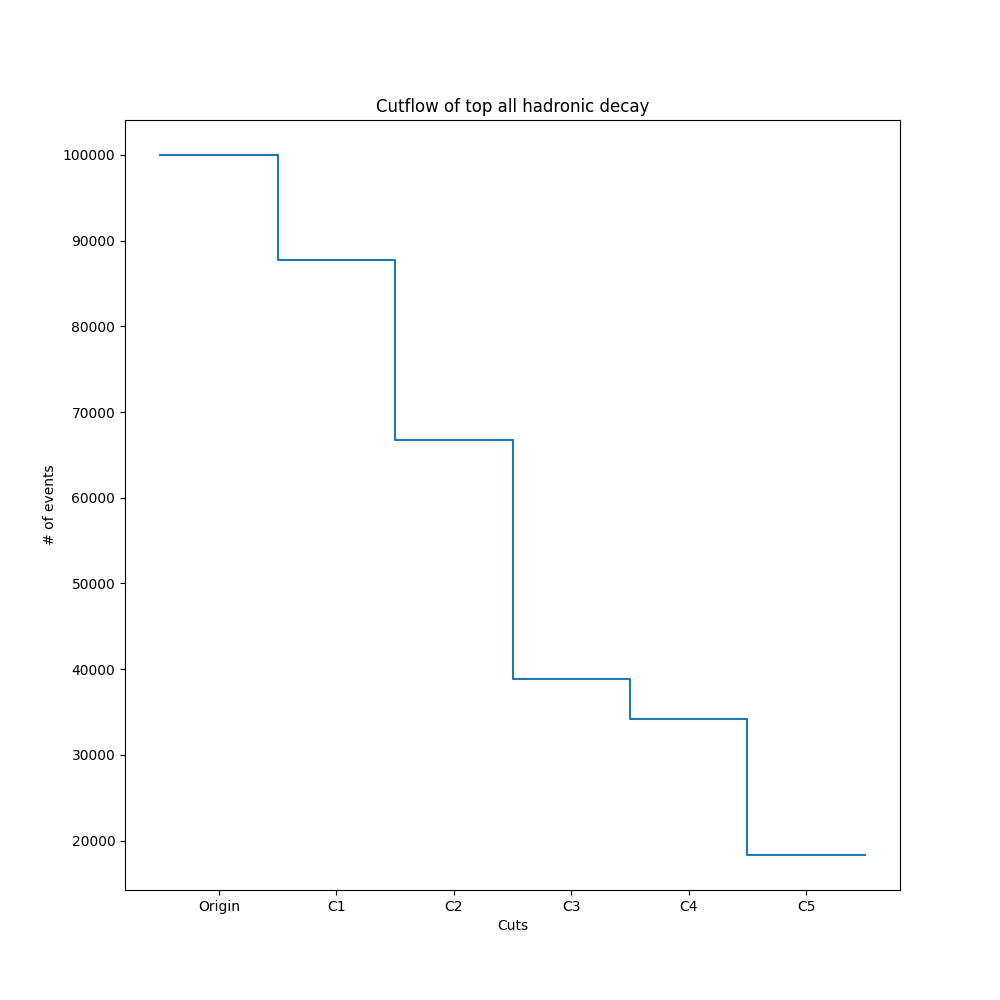
\includegraphics[width=0.9\linewidth]{Figures/ttbar_cutflow.png}
	\caption{Cutflow of all hadronic top decay.}
	\label{fig:cutflow}
\end{figure}
\subsection{Truth matching}\label{subsec:Truth matching}
The \textbf{truth matching}, which is also called \textbf{$\Delta$R matching},  is to match the detector simulation(i.e. jet information generate by Delphes) data to truth record(i.e. Parton level information).  To calculate the $\Delta R$ value, we will find the daughters of top quarks, W boson, and b quark. After the daughters of top quarks are found, we will find the daughters of W bosons. Finally, we will get six partons that come from the decay of top quark pairs. These six partons can match the jets identically by considering their distances. The formula of calculating $\Delta R$ is:
\\
\begin{equation}
	\Delta R = \sqrt{\Delta\eta^{2} + \Delta\phi^{2}}
\end{equation}
By using the kinematic properties provided in parton level and detector simulation information, we can calculate the $\Delta R$ value between each parton and jets. Using the result of the calculation, we may assign each parton to a specific jet. 
\\
\subsection{Custom barcode system}\label{subsec:barcode}
To specify the relation between each parton, and the relation between mothers and daughters, we design a barcode system that helps us to declare the relationship.
\begin{figure}[H]
	\centering
	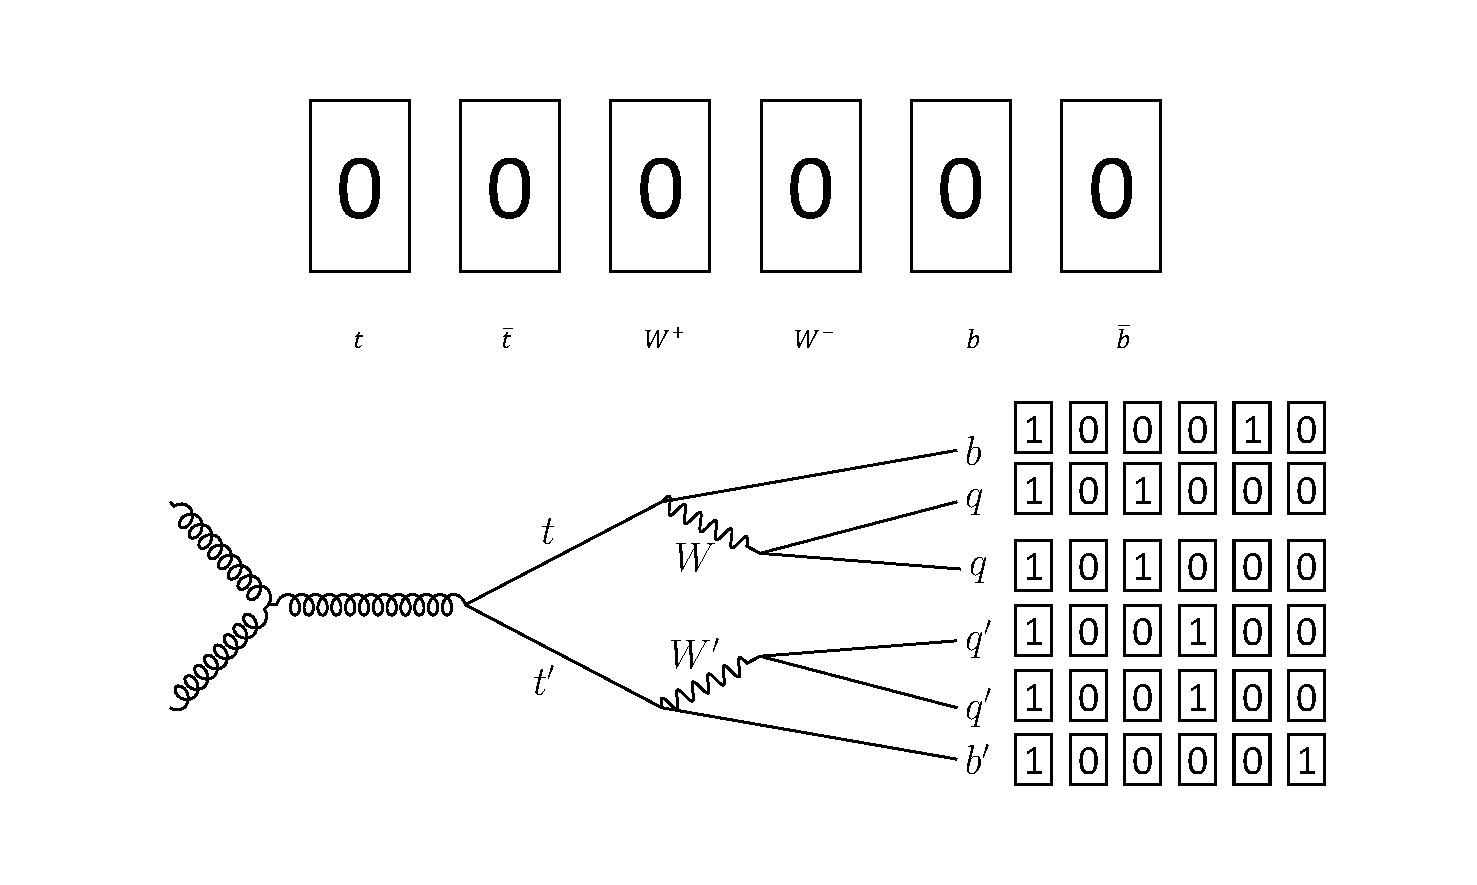
\includegraphics[width=1.1\linewidth]{Figures/barcode.pdf}
	\caption{Design of barcode. These barcodes can provide a pari-wide information to our network.}
	\label{fig:barcode}
\end{figure}
\newpage
In Figure \ref{fig:barcode}, we define a six-digit barcode, the first two digits are to show which top quark is the mother of this parton, the last four digits of the sequence are to declare which daughter of the top quark is the mother of parton. In this case, we can use this barcode system to break six parton(jet) candidates into two subsets which contain 3 elements. The benefit of using this barcode system is not only to specify the relation without losing the information, but also provide a permutation relationship to our network. We will discuss this in the following section.
\section{Event reconstruction}\label{sec:Event reconstruction}
\subsection{$\chi^{2}$ minimization method}\label{subsec:chi-square}
The $\chi^{2}$ minimization method is a traditional method to reconstruct an event. For an event that exists 6 jets, it has about $6!/(2\times2\times2)=90$ possible combinations, the first two in the denominator is contributed by two b-tag jets, and the middle one and last one is the contributions from two pairs of quark produce by W bosons. The number of possible combinations is proportional to the number of existing jets in an event. The $\chi^{2}$ minimization method will calculate all the candidates and try to find the candidate which has the smallest $\chi^{2}$ value. This method based on the mass of the W boson and top quark. The origin equation of $\chi^{2}$ minimization in this model is:
\begin{equation}\label{eqn:chi2}
	\chi^{2} = \frac{( m_{bqq'} - m_{t} )^{2}}{\sigma_{t}^{2}} + \frac{( m_{\bar{b}q''q'''} - m_{t} )^{2}}{\sigma_{t}^{2}} + \frac{(m_{qq'} - m_{W})^{2}}{\sigma^{2}_{W}} + \frac{(m _{q''q'''} - m_{W})^{2}}{\sigma^{2}_{W}}
\end{equation} 
The equation \ref{eqn:chi2} has four part. Each parts is a ``pull'' that is contributed by the component of observables. The parameter $\sigma_{W}$ and $\sigma_{t}$ is obtained by applying a fitting to the distribution of reconstructed invariant mass of W boson and top quarks. And the mass of the W boson and top quark is given by the recent experiment result. To avoid the bias of top quark candidates, we may combine the first two term into one term by substituting $m_{t}=\frac{m_{bqq'} + m_{\bar{b}q''q'''}}{2}$, then the equation reduces to: 
\begin{equation}\label{eqn:chi2_mod}
	\chi^{2} = \frac{(m_{bqq'} - m_{\bar{b}q''q'''})^{2}}{\sigma^{2}_{\Delta_{m_{bqq'}}}}  + \frac{(m_{qq'} - m_{W})^{2}}{\sigma^{2}_{W}} + \frac{(m _{q''q'''} - m_{W})^{2}}{\sigma^{2}_{W}}
\end{equation} 
Note that there are some events the three-jets invariant mass can be far away from the top quark mass but still give us a small $\chi^{2}$ value. This is because we only consider the difference between two three-jets invariant mass. This can be improved by applying a constraint to the invariant mass\cite{Mccarthy:2015ucy}, but we didn't apply such a constraint in this report. 
\\
In this project, we force the b quark candidates in equation \ref{eqn:chi2_mod} must be b-tagged jets. This may help to reduce the number of permutations but prevent the event that contains a jet mistagged be assigned correctly.
\subsection{Machine Learning Approach}\label{subsec:ML approach}
For a machine learning model, equivariance and invariance are important properties that may affect the performance of the model. Such as a computer vision problem, the object should be invariant under translation to prevent affect the prediction. The translation, rotation, and shift of the position should not change the prediction of the model because the object remains the same object. The Convolutional Neural Network(CNN) can produce object recognition outcomes that are invariant under translations. The properties of invariance can be generalized to another geometry structure, e.g. manifolds and groups. In all hadronic top decay, we have two subsets with the same elements $(b, q, q')$ and $(\bar{b}, q'', q''')$. These subsets should remain invariant under permutations of the input jets order. The reason that the order of input jets should not affect the result is because the permutation symmetry is not base on the order of jets but the pair-wise permutation.
\\
By the invariant feature of attention architecture, rearranging the elements in a sequence leaves the attention weight unchanged. We may use this permutation symmetry present in the attention-based model to handle the reconstruction of all hadronic top decay process efficiently. In this case, the network output of the all hadronic top decay process should identify two distinct interchangeable subsets, and each contains an interchangeable $qq'$ pair produced by the W bosons. This invariant property on the output is the unique feature of our dataset and the model should take into account. 
\\
We propose an attention-based network, called \textbf{Symmetry Preserving Attention NETwork(SPA-NET)} in this project. Its structure is shown in Figure \ref{fig:architecture}}. The input of SPA-NET is a list of unsorted jet information, with their 4-momentum $(p_{\rm T}, \eta, \phi, M)$ as well as the b-tag information provided by Delphes. We take the logarithm to $M$ and $p_{T}$ and normalize all the components to have zero mean and unit variance.  The input jets will be sent to the network and be embedded into a D-dimensional latent space representation. This D-dimensional latent space is obtained by progressively increasing the latent dimensionality of the input jets up to the final dimensionality D(This operation is done by the embedding blocks in the whole stack). We target this latent space dimensionality D to a value 128 with the following sequence: 8 $\to$ 16 $\to$ 32 $\to$ 64 $\to$128.  After embedding, the output will be sent to a stack of transformer encoder layers, this layer will learn the relationship between each element in the input sequence. While the encoding is finished, the encoded output will be forwarded into an important architecture in this network, a two branches structure that computes the output individually. There is a transformer encoder in each branch, this encoder layer will extract the information of the top quark and the tensor attention layer will produce the top quark distribution. The output distribution predicts the top quark triplets. Figure \ref{fig:output} is an example of network outputs. Note that the attention mechanism is an architecture that allows the network to propagate the information selectively by using a  ``mask''. By the implementation of the mask, the neural network can learn from partial information and update the parameters with selected information, and allow the network to infer the relationships between different elements in a sequence.
\\
\begin{figure}[H]
	%\captionsetup{justification=raggedright,singlelinecheck=false}
	\centering
	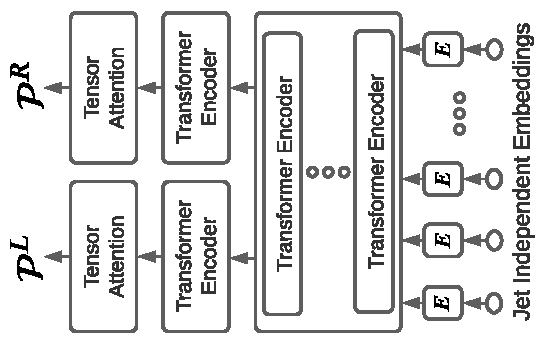
\includegraphics[width=0.48\textwidth,angle=270]{Figures/NetworkDiagramAlt.pdf}
	\caption{ High-level structure of SPA-NET.}
	\label{fig:architecture}
\end{figure}
\begin{figure}[H]
	%\captionsetup{justification=raggedright,singlelinecheck=false}
	\centering
	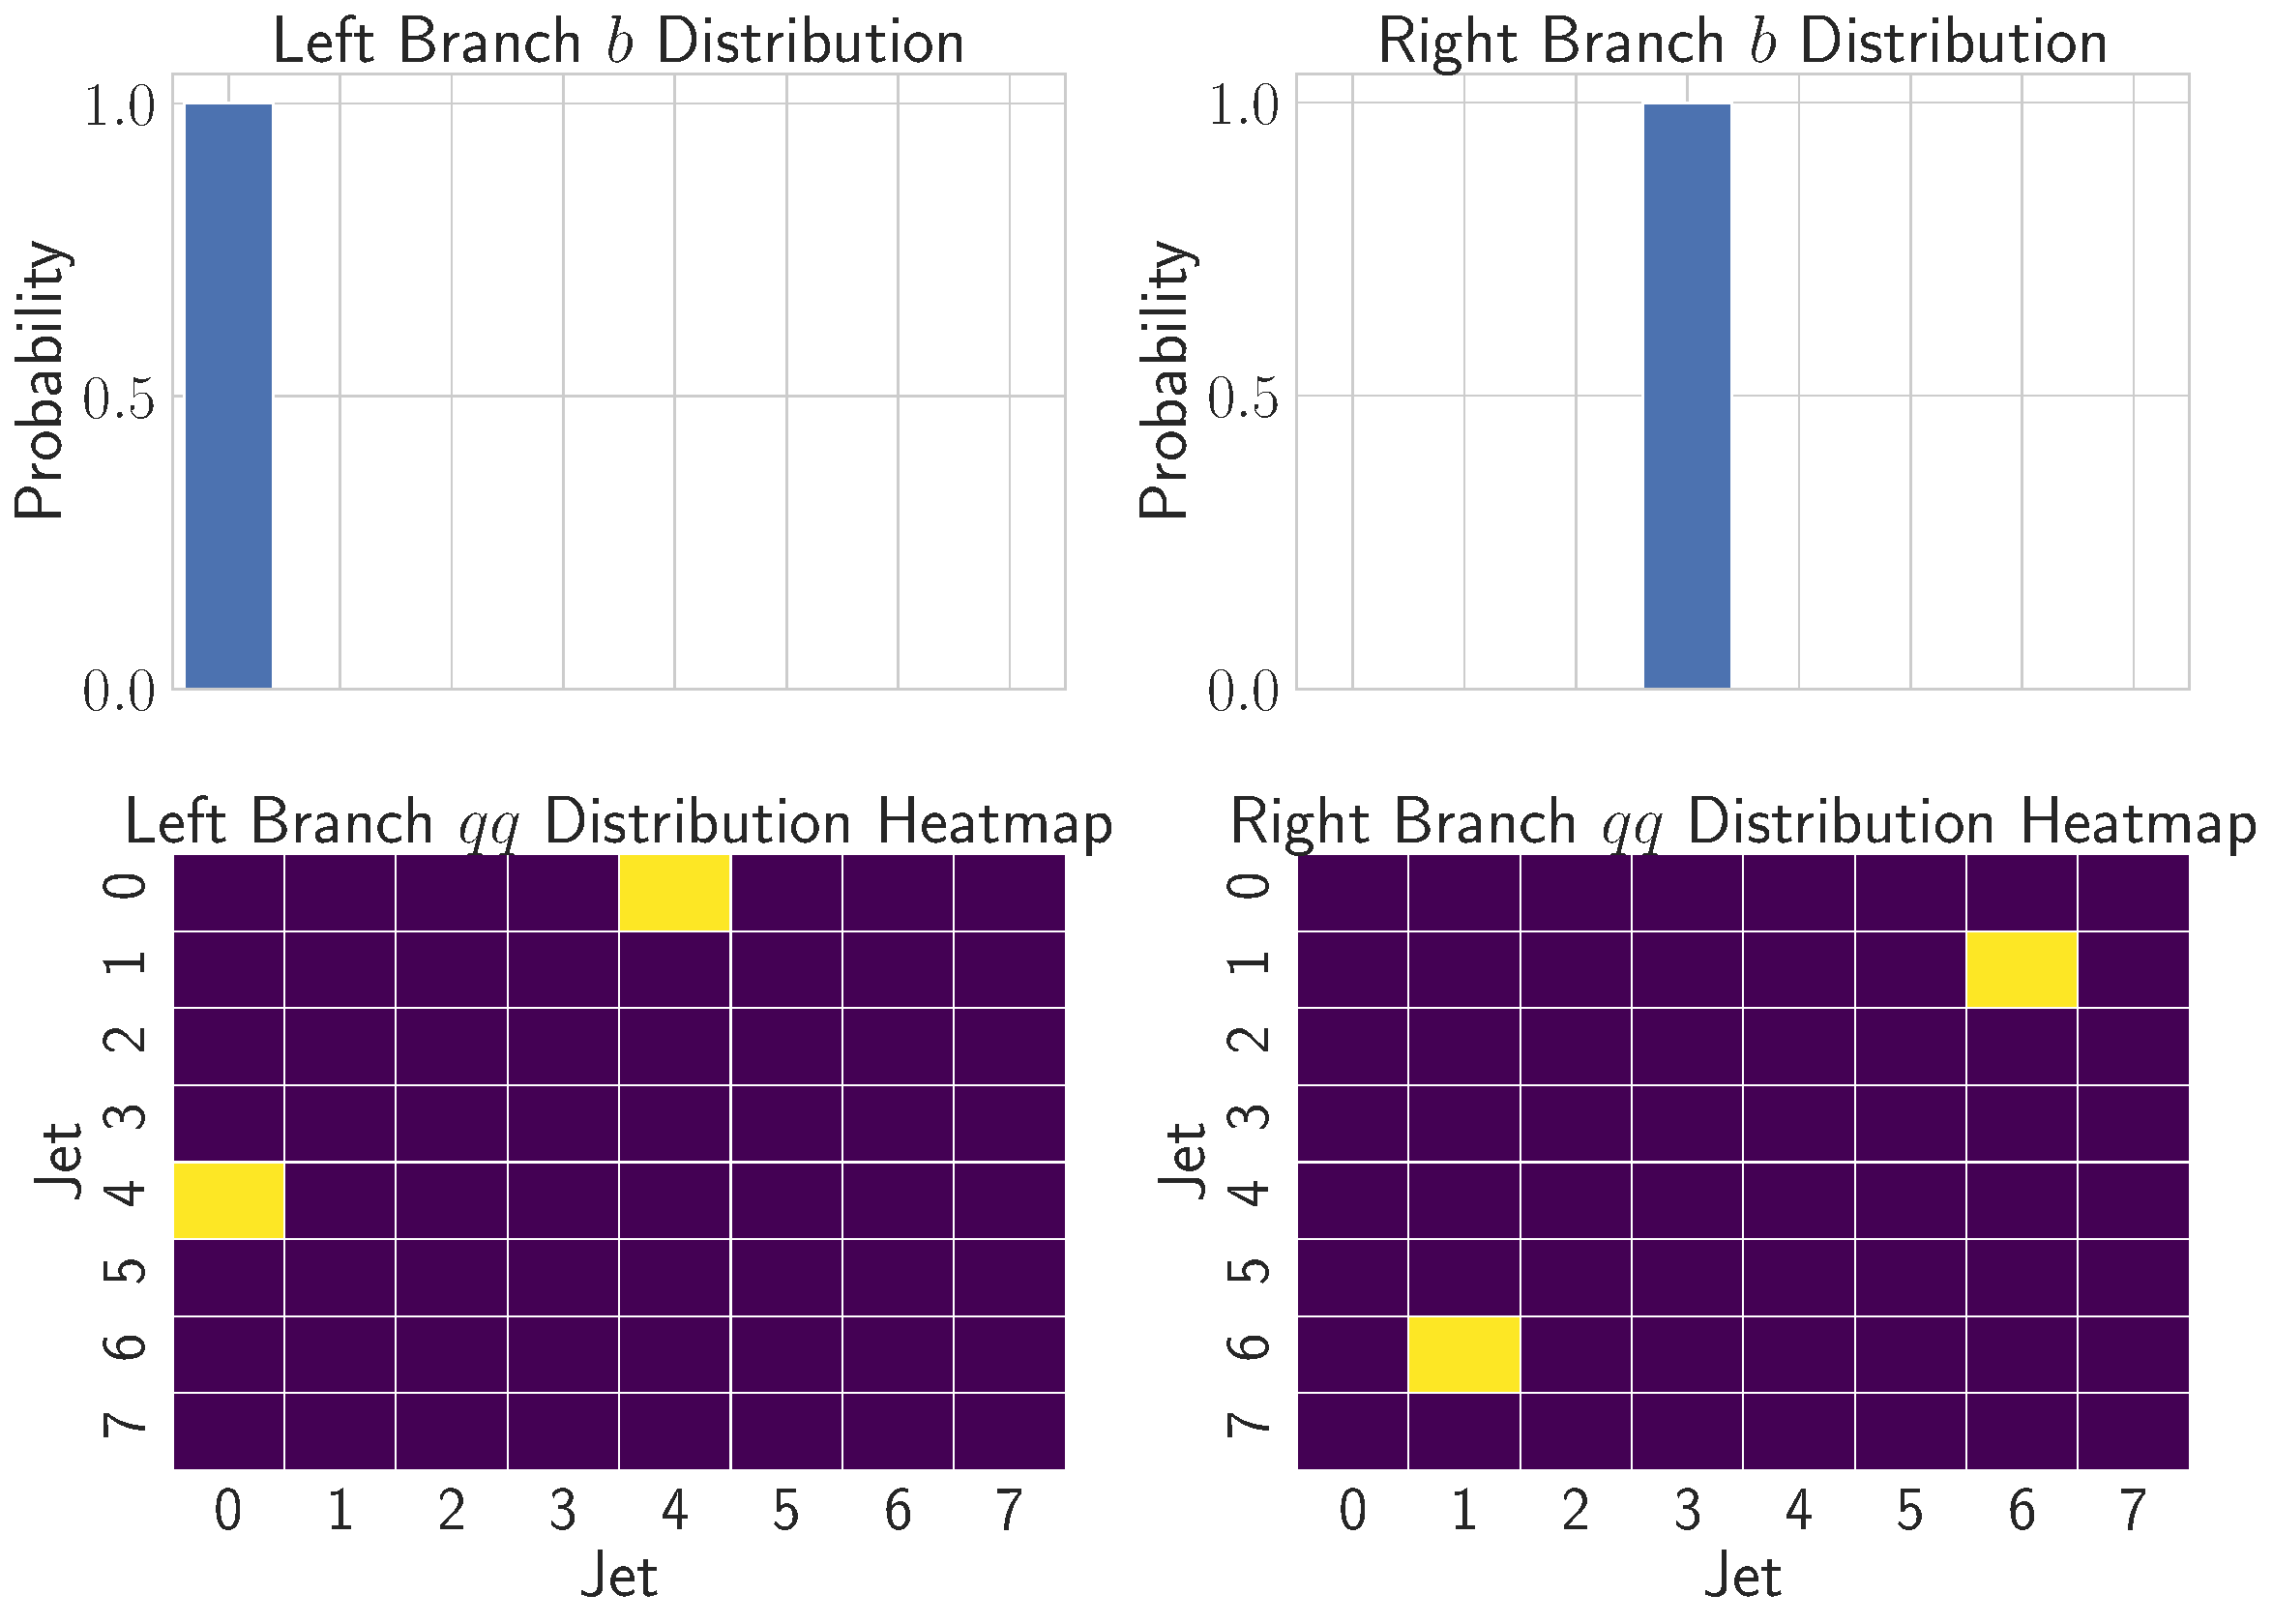
\includegraphics[width=0.8\textwidth]{Figures/typical_output.pdf}
	\caption{A visualization of the example single event output produced by SPA-NET. The top two plots are the projected b quark distribution, and the bottom two plots are the qq′ distribution respectively. }
	\label{fig:output}
\end{figure}
The most important part in this network is the \textbf{Symmetry Preserving Tensor Attention}. Consider a set of weights $\theta \in \mathbb{R}^{D\times D\times D}$, this $\theta$ is not inherently symmetric at all. To make the $\theta$ become an invariant attention weighting, we apply the following transformation(eq. \ref{eqn:SPTA}). This transformation will transform the $\theta$ into an auxiliary weights tensor $S^{ijk}\in R^{D\times D\times D}$. Using $S^{ijk}$ and the embedded jets tensor $X \in \mathbb{R}^{N\times D}$(N is the number of jets), we can calculate the dot-product attention. The dot-product works in flat Euclidean space and produces the output tensor $O^{ijk}$. The summation product tensor $S^{ijk}$ guarantees the interchangeable of the first two dimensions of $S$ will be symmetric and ensures that $O^{ijk}=O^{jik}$. These properties enforce the $qq'$ invariance.
\\
\begin{equation}\label{eqn:SPTA}
	\begin{split}
	S^{ijk} &= \frac{1}{2}\left( \theta^{ijk} + \theta^{jik}\right) \\
	O^{ijk} &= X^{i}_{n}X^{j}_{m}X^{k}_{l}S^{nml}
		\end{split}
\end{equation}
\\
To obtain the probability distributions $P^{L}$ and $P^{R}$, we apply a 3-dimensional softmax on $O^{ijk}$ to generate the joint triplet probability distribution.
\\
\begin{equation}\label{eqn:PDF}
	P(i,j,k) = \frac{exp\ O^{ijk}}{\sum_{ijk} exp\ O^{ijk}}
\end{equation}
\\
We use equation \ref{eqn:PDF} to produce the individual probability distribution of two top quarks and produce the single triplet from each by selecting the peak of these distributions. 
\\
During the training, a suitable loss function is needed to deal with the double output probability distributions. We design the loss function based on the cross-entropy between the output probability and truth distribution on the all hadronic top decay. The loss function must ensure the symmetry of the top quark pairs which are invariant concerning the permutation $tt' \leftrightarrow t't$.  We create a symmetry loss function $\mathcal{L}$ by the following function:
\\
\begin{align}
		&\mathcal{L} = min(\mathcal{L}_{1}(P^{L}, T_{1}, P^{R}, T_{2}), \mathcal{L}_{1}(P^{L}, T_{2}, P^{R}, T_{1})) \\
		&\mathcal{L}_{1}(P_{1}, T_{1}, P_{2}, L_{2}) = \mathcal{H}(T_{1}, P_{1}) +\mathcal{H}(T_{2}, P_{2})
\end{align}
\\
Where the $\mathcal{H}$ is the general cross-entropy. It is possible that both branches produce the same output pairs. To make sure the network produces unique predictions, we will select the higher probability one and re-evaluate the other one, then compute the loss function. The Figure \ref{fig:output} is an example of the output produced by SPA-NET.










